\chapter{Basics} \label{Chapter 2}
\label{chap:first chapter}

The aim of this project is to study and devise an advanced control method, in this case model predictive control (MPC), for a highly non-linear system with an unstable equilibrium, in this case an inverted pendulum.
As the name suggests, model predictive control involves the mathematical model of the system. By solving an optimization problem using states that are fed back to the this model, one can predict the optimal state trajectory for the next $\mathnormal{N}$ time steps. This $\mathnormal{N}$ is called the prediction horizon of the controller and is an important parameter that can be tuned for better performance.

In this chapter we will look at the mathematical modelling of this system as well some basic MPC theory that enables one to design a stable and optimal controller. 

\section{Inverted pendulum}
The inverted pendulum or the "cart-pole" system, as mentioned before is a standard test case for new control strategies. For MPC it is first important to model this system mathematically, the following section gives an brief overview of the real system followed by the mathematical modelling of this system.

\subsection{Physical System}

The outer construction of the pendulum, as shown in Figure \ref{fig: Outer covering}, consists of extruded aluminium and custom-designed elements made of PET-G material. The internal components, shown in Figure \ref{fig: Internal components} are also custom-designed and made of either PET-G or PLA+ \cite{PendulumManual}.

The internal components consist of the following:
\begin{itemize}
	\item Pendulum connector : Connects the pendulum arm to the cart.
	\item Rotary encoder :To measure the angle of rotation of the pendulum arm.
	\item Cart rails : For cart movement.
	\item Motor : A stepper motor which moves the cart.
	\item Motor driver : Used to control the stepper motor. 
	\item MCU : The ESP32 microcontroller unit responsible for generating the PWM signal for the motor.
	\item Limit switches : 2 limit switches at either side of the cart mark the limits of the cart.
\end{itemize}


\begin{figure}[H]
	\centering
	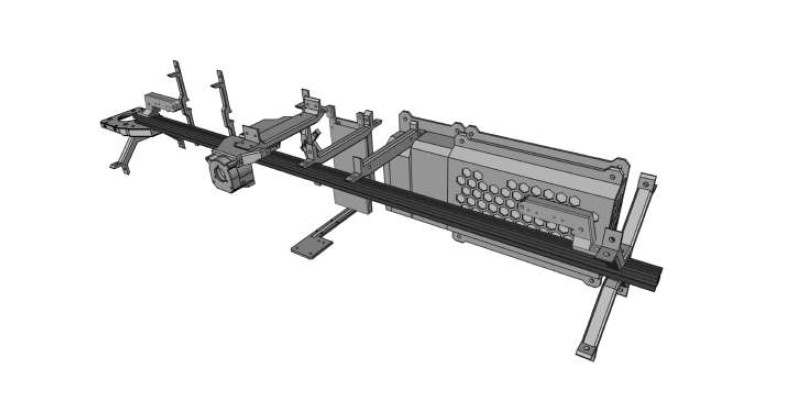
\includegraphics[width=0.75\textwidth]{"src/Images/Pendulum_inner.jpg"}
	\caption{internal components \cite{PendulumManual}.}
	\label{fig: Internal components}
\end{figure}

\begin{figure}[h!]
	\centering
	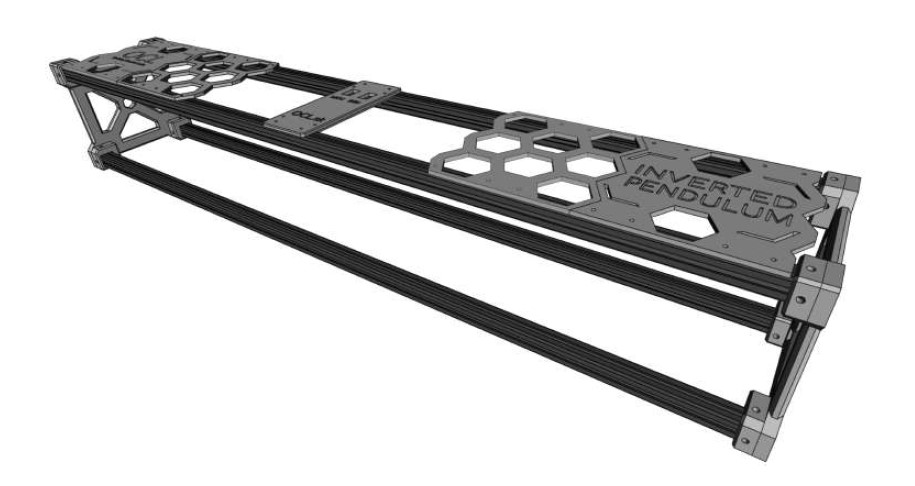
\includegraphics[width=0.75\textwidth]{"src/Images/Pendulum_outer.jpg"}
	\caption{outer covering \cite{PendulumManual}.}
	\label{fig: Outer covering}		
\end{figure}


\begin{figure}[H]
	\centering
	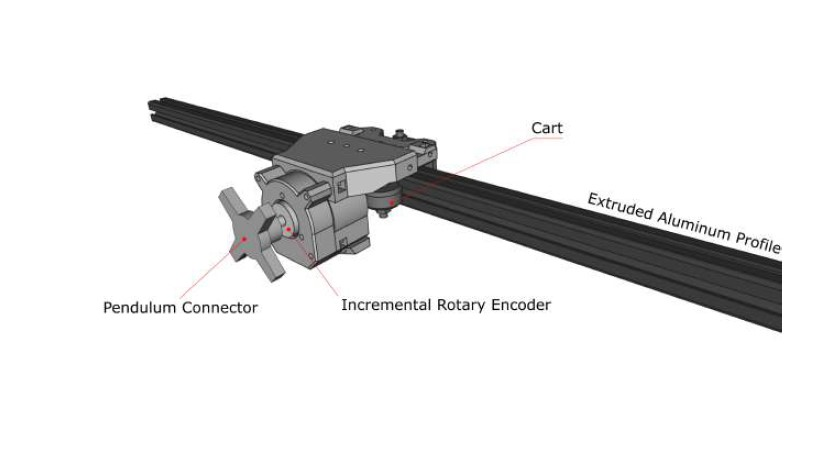
\includegraphics[width=0.75\textwidth]{"src/Images/Pendulum_cart.jpg"}
	\caption{pendulum cart and rotary encoder \cite{PendulumManual}.}
	\label{fig:Pendulum Cart}
\end{figure}  

\begin{figure}[H]
	\centering
	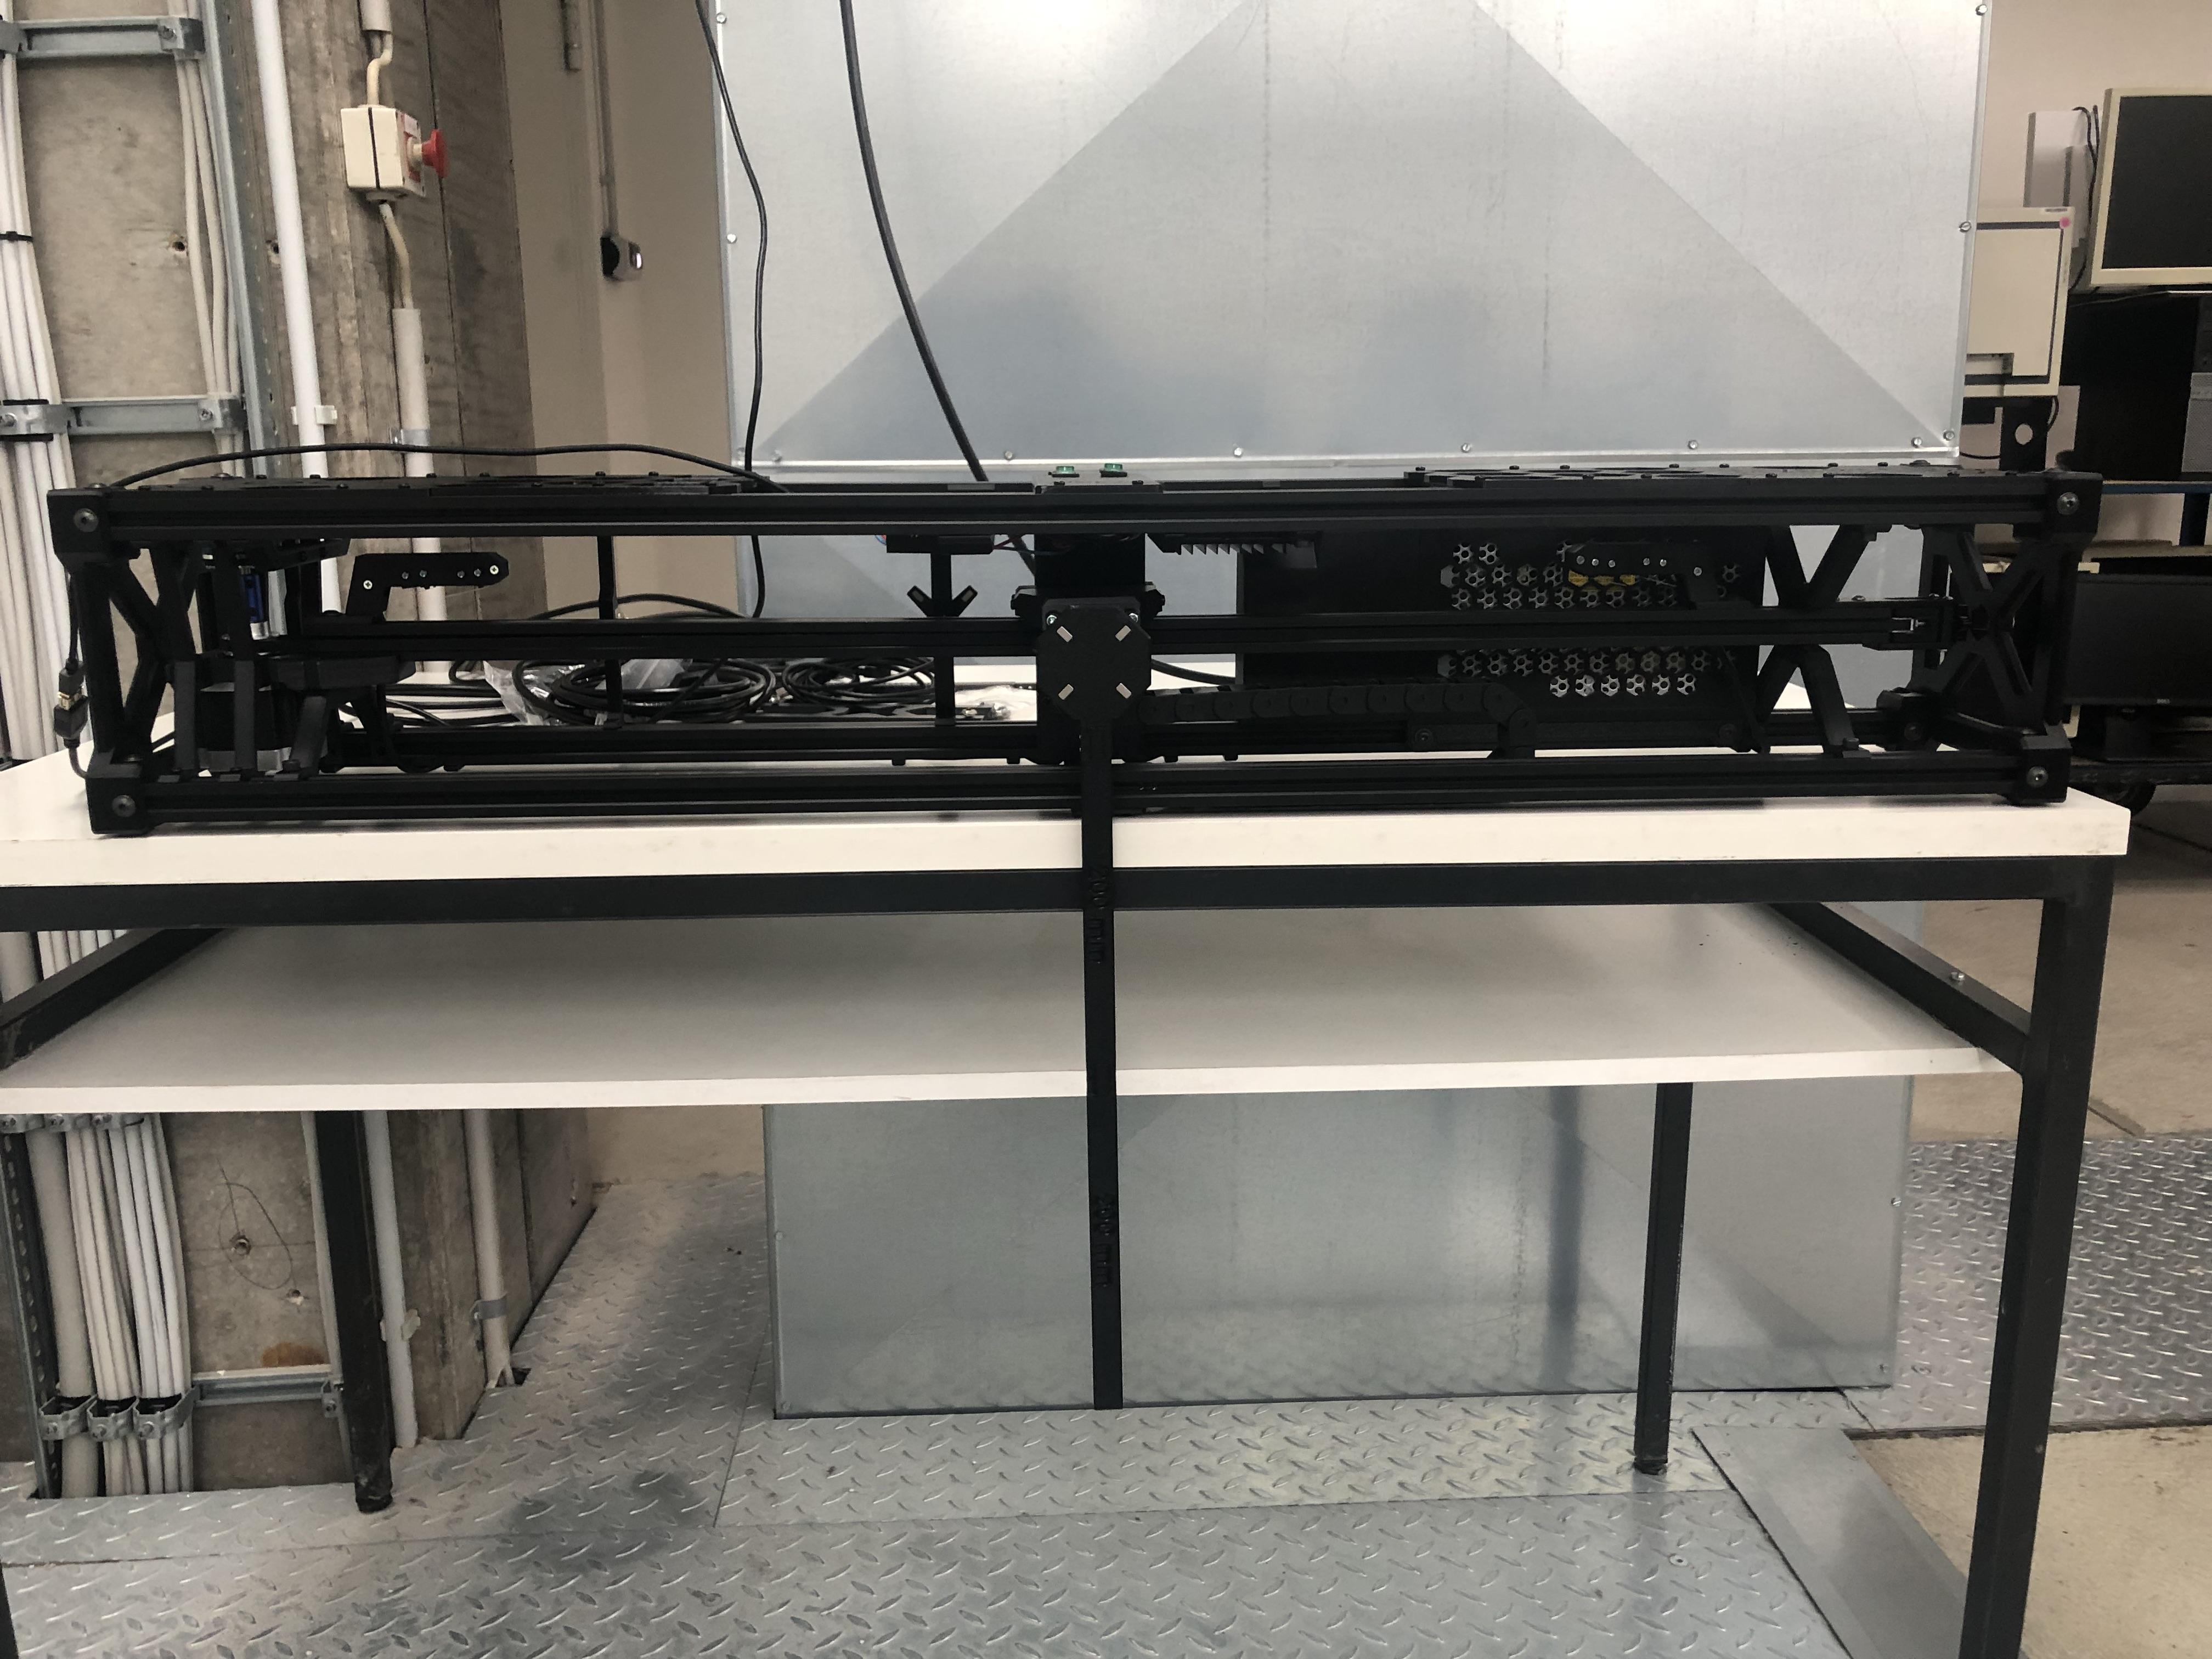
\includegraphics[width=0.75\textwidth]{"src/Images/Real_pendulum1.jpg"}
	\caption{inverted pendulum : front view}
	\label{fig:Real Pendulum}
\end{figure}  


\begin{figure}[h!]
	\begin{subfigure}{0.5\textwidth}
		\centering
		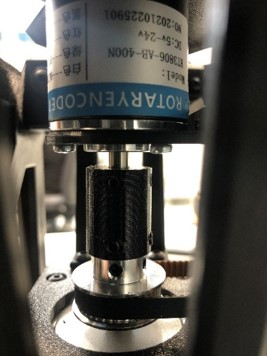
\includegraphics[width=0.6\textwidth]{"src/Images/Motor.jpg"}
		\subcaption{motor and encoder.}
		\label{fig:Motor}
	\end{subfigure}
	\hfill
	\begin{subfigure}{0.7\textwidth}
		\centering
		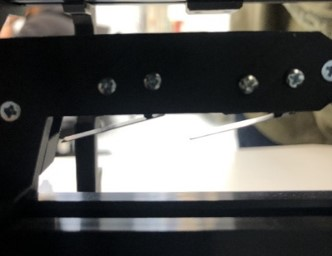
\includegraphics[width=0.6\textwidth]{"src/Images/Limit_Switch.jpg"}
		\subcaption{limit switch.}
		\label{fig:Limit Switch}
	\end{subfigure}
	\caption{pendulum components: motor and limit Switch.}
	\label{fig:Components of the Pendulum : Motor and Limit Switch}
\end{figure}


\begin{figure}[h!]
	
	\begin{subfigure}{0.45\textwidth}	
		\includegraphics[width=\textwidth,scale=0.75]{"src/Images/Real_pendulum3.jpg"}
		\subcaption{ESP32 microcontroller}
		\label{fig:ESP32 Microcontroller}
	\end{subfigure}
	\hfill
	\begin{subfigure}{0.45\textwidth}
		\centering
		\includegraphics[width=\textwidth,scale=0.75]{"src/Images/Real_pendulum4.jpg"}
		\subcaption{motor driver}
		\label{fig:Motor Driver}
	\end{subfigure}
	\caption{pendulum components: microcontroller and driver}
	\label{fig:Components of the Pendulum: Driver and ESP}
\end{figure}  

The motor is controlled using a motor driver and an ESP32 microcontroller, shown in Figure \ref{fig:Components of the Pendulum: Driver and ESP}, that produces Pulse Width Modulated (PWM) signals to control the step angle to produce desired velocities. Since the input chosen was the cart acceleration, we have to first convert this to the cart velocity at current time. This can be done using the relation,  $$v_{cart} = u\cdot dt + v_0 $$ 
where $u$ is the cart acceleration, dt is the sampling time of the pendulum and $v_0$ is the velocity at the previous time step. This is then converted to the frequency of the PWM signal using the relation
$$f_{pwm} = v_{cart}\cdot20,000$$
This is explained in more detail in later chapters. 

\subsection{Mathematical Model} 

We first start by defining a few variables and what they represent in our inverted pendulum system : 	
\begin{itemize}
	\item Cart position: $x(t)$
	\item Pendulum centre of gravity x-Position: $x_s(t)$
	\item Pendulum centre of gravity y-Position: $y_s(t)$
	\item Pendulum angle measured from the top equilibrium: $\theta(t)$
	\item Pendulum length: $\ell$
	\item Pendulum mass: $m$
	\item Pendulum moment of inertia: $J = m\ell^2 / 12$
	\item Angular friction coefficient: $b$
	\item Contact forces between pendulum and cart: $F_x(t), F_y(t)$
	\item Gravity constant: $g$
\end{itemize}

\begin{figure}[htbp]
	\centering
	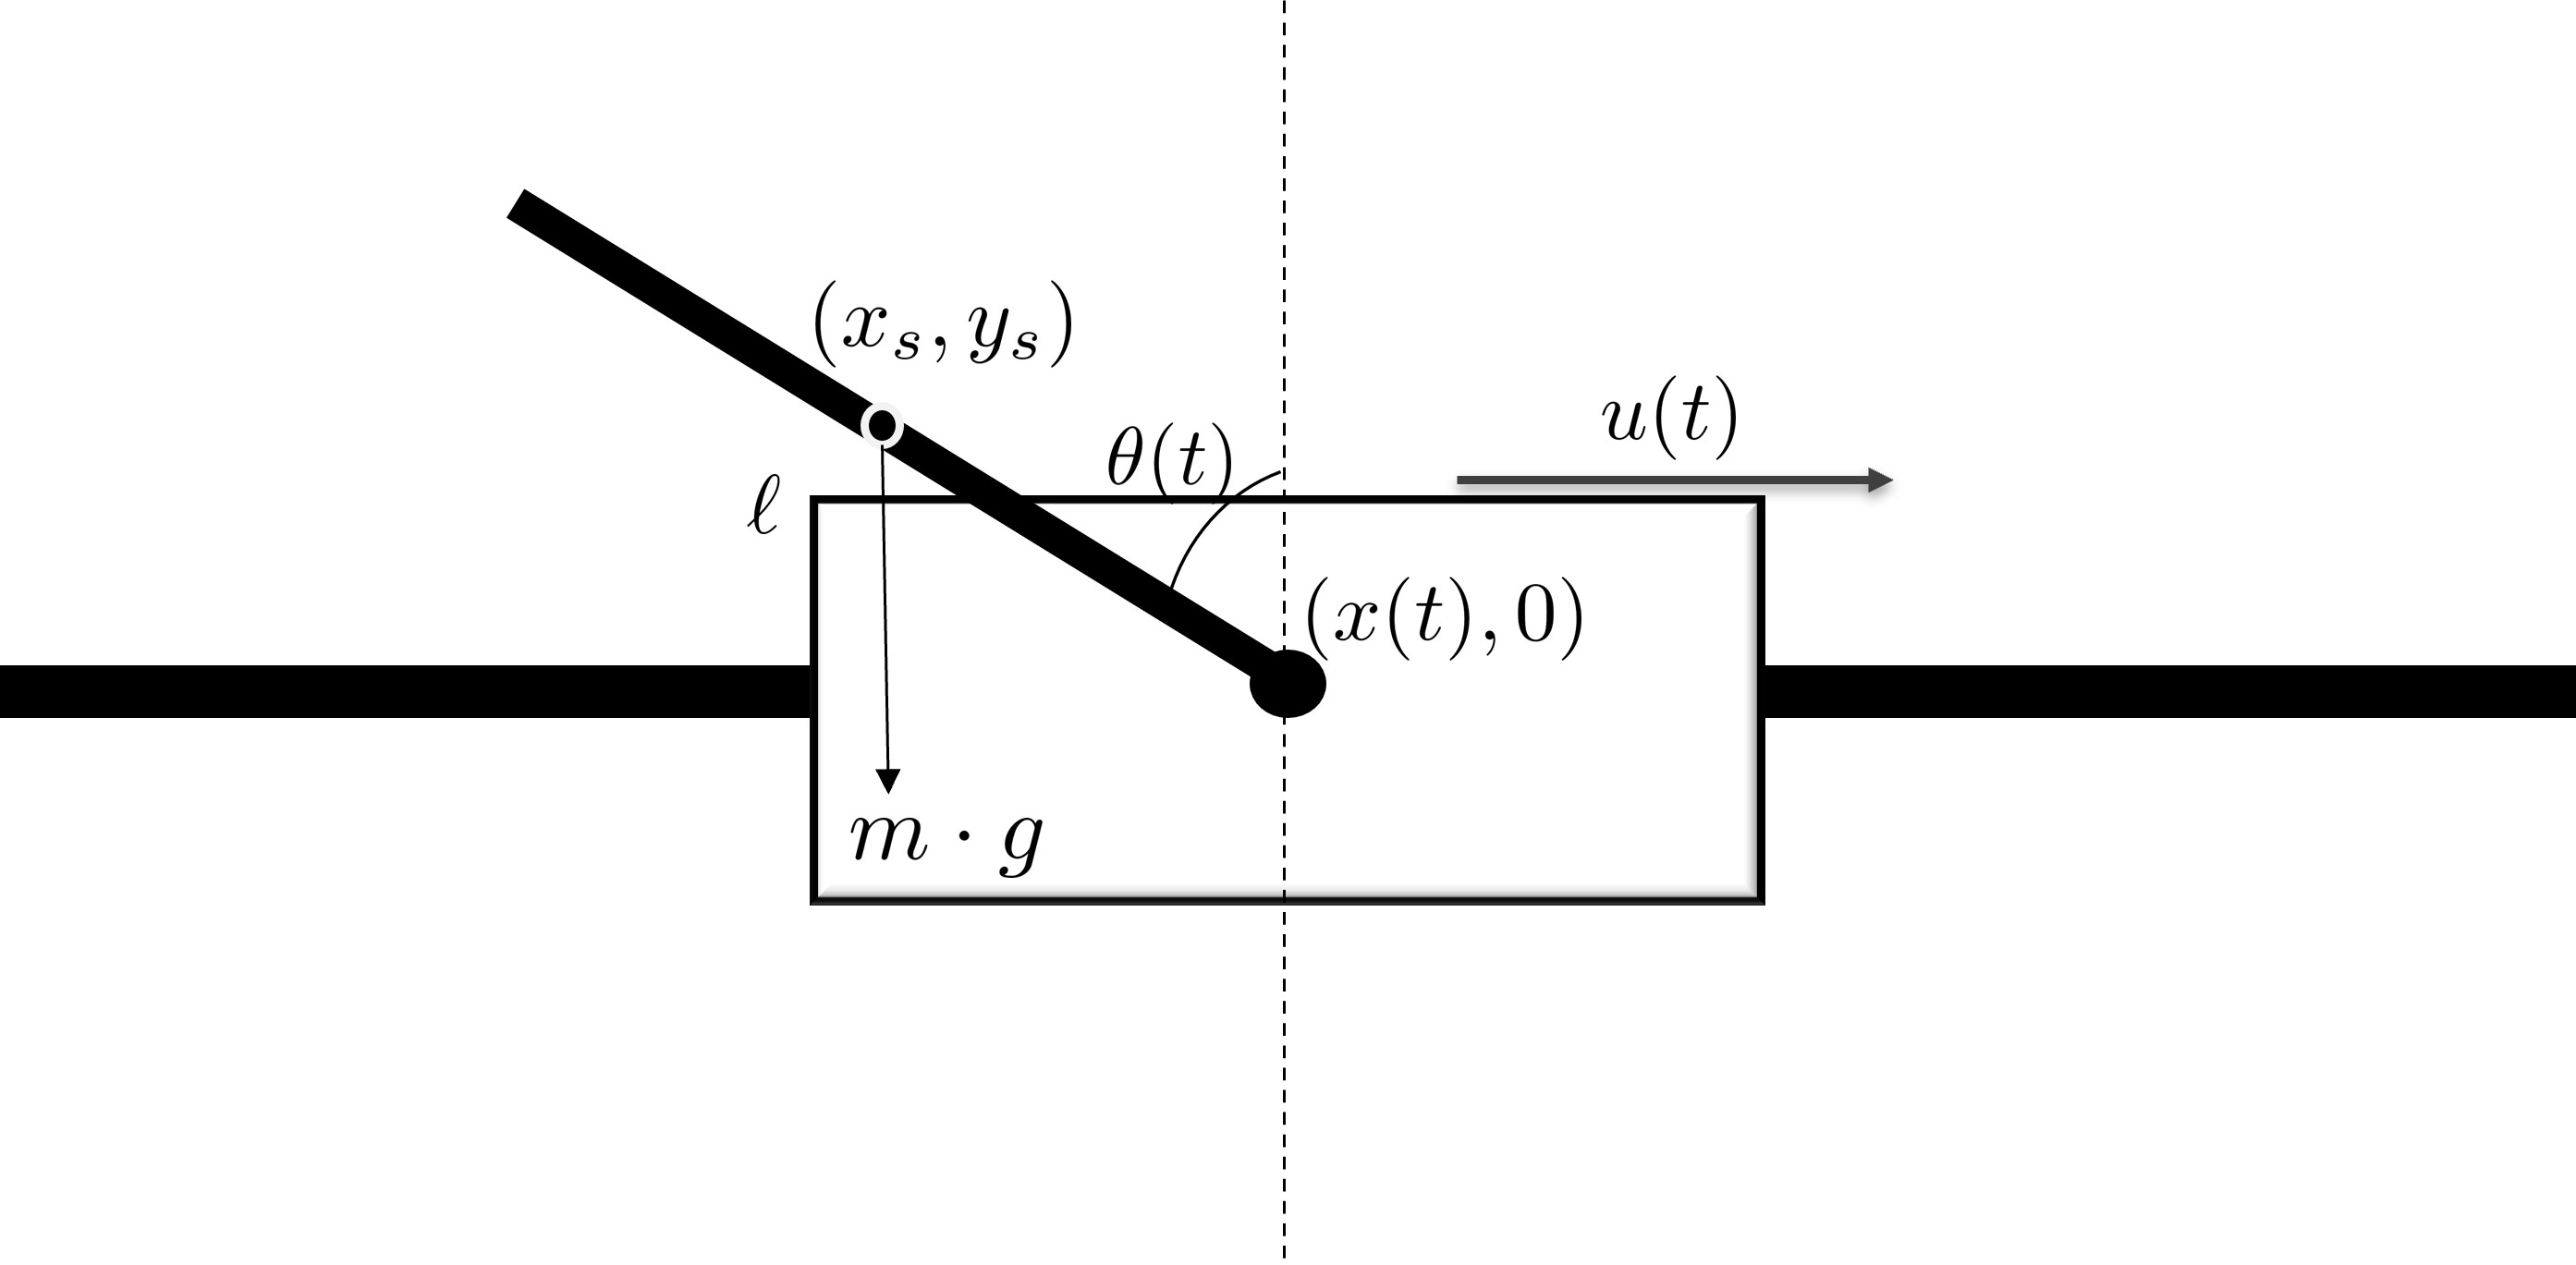
\includegraphics[width=0.5\textwidth]{"src/Images/pendulum1.jpg"}   
	\caption{pendulum schematic}
	\label{fig:Pendulum schematic}
\end{figure}


We then define the coordinates,linear velocity and acceleration of the centre of gravity of the pendulum arm as $(x_s,y_s)$, $(\dot{x}_s, \dot{y}_s)$ and $(\ddot{x}_s,\ddot{y}_s)$ respectively. These can then be calculated as follows:


\begin{align*}
x_s &= x - \frac{\ell}{2} \sin(\theta)\\
\dot{x}_s &= \dot{x} - \frac{\ell}{2}\dot{\theta}\cos(\theta)\\
\ddot{x}_s &= \ddot{x} - \frac{\ell}{2}\ddot{\theta}\cos(\theta) + \frac{\ell}{2}\dot{\theta}^2\sin(\theta)\\
y_s &= \frac{\ell}{2}\cos(\theta)\\
\dot{y}_s &= -\frac{\ell}{2}\dot{\theta}\sin(\theta)\\
\ddot{y}_s &= -\frac{\ell}{2}\ddot{\theta}\sin(\theta)- \frac{\ell}{2}\dot{\theta}^2\cos{\theta}
\end{align*}



In first principle modelling one uses basic physical conservation laws to model the system, in chemical reactors for example, one can use molar balance equations. In this case we use force balance equations.

So applying force balance in x-direction of the pendulum we get:
\begin{equation}\label{eq:xbalance}
m \ddot{x}_s = F_x
\end{equation}

Similarly, applying force balance in y-direction of the pendulum, we get:
\begin{equation}\label{eq:ybalance}
m \ddot{y}_s = F_y - mg
\end{equation}

Another possible quantity that can be balanced is torque, so applying torque balance to the pendulum's centre of gravity (CoG), we obtain:
\begin{equation}\label{eq:torquebalance}
J\ddot{\theta} = F_x \frac{\ell}{2}\cos(\theta) + F_y \frac{\ell}{2}\sin(\theta) - b\dot{\theta}
\end{equation}

Plugging~\eqref{eq:xbalance} and~\eqref{eq:ybalance} into~\eqref{eq:torquebalance} to obtain

\begin{equation}\label{eq: 2.4}
\left(J + m\frac{\ell^2}{4} \right) \ddot{\theta} = m \ddot{x} \frac{\ell}{2}\cos(\theta) + mg \frac{\ell}{2}\sin(\theta) - b\dot{\theta}
\end{equation}
Since $J = m\ell^2 / 12$ we get $(J + m\ell^2/4) = m\ell^2/3$. This results in a reformulated equation which reads:
\begin{equation}
\ddot{\theta} = \frac{3 \cos(\theta)}{2 \ell} \ddot{x} + \frac{3 \sin(\theta)}{2\ell} g - \frac{3b}{m\ell^2} \dot{\theta}
\end{equation}

\begin{equation}
\begin{aligned}
\ddot{\theta} &= \frac{3g}{2\ell} \sin(\theta)    -\frac{3b}{m\ell^2} \dot{\theta}              + \frac{3}{2\ell} \cos(\theta)u\\
\ddot{x} &= u 
\end{aligned}
\end{equation}

We can also redefine the friction coefficient $b'=\frac{3b}{m\ell^2}$, with this we get

\begin{equation}
\begin{aligned}
\ddot{\theta} &= \frac{3g}{2\ell} \sin(\theta)    -b' \dot{\theta}              + \frac{3}{2\ell} \cos(\theta)u\\
\ddot{x} &= u. 
\end{aligned}
\end{equation}

\vspace{0.5cm}

from the above derivation of the system model, one can decide on the states, inputs and outputs of the inverted pendulum model as follows : 

\begin{itemize}
	\item States: 
	\begin{itemize}
		\item $x_1(t) \doteq \theta(t)$  - angular displacement of pendulum
		\item $x_2(t) \doteq \dot{\theta}(t)$ - angular velocity of the pendulum
		\item $x_3(t) \doteq x(t)$    - linear displacement of the cart
		\item $x_4(t) \doteq \dot{x}(t)$ - linear velocity of the cart
	\end{itemize}
	\item Input:
	\begin{itemize}
		\item $u(t) \doteq \ddot{x}(t)$ i.e. input = cart acceleration
	\end{itemize}
	\item Measured quantities: 
	\begin{itemize}
		\item $x_1(t)$ from pendulum encoder
		\item $x_3(t)$ from cart encoder
	\end{itemize}
\end{itemize}

And so the full dynamic equation of the inverted pendulum can be written as 

\begin{equation}
\begin{bmatrix}
\dot{x}_1 \\
\dot{x}_2 \\
\dot{x}_3 \\
\dot{x}_4
\end{bmatrix} = \begin{bmatrix}
x_2\\
\frac{3g}{2\ell} \sin(x_1)    -\frac{3b}{m\ell^2}x_2              + \frac{3}{2\ell} \cos(x_1)u \\
x_3 \\
u
\end{bmatrix}
\end{equation}



\section{Model Predictive Control}

As mentioned before, model predictive control is a very popular strategy among other advanced control methods. There are many reasons for its popularity, some being that it is able to consider the entire non-linear system without any linearising approximations and it is also very adept at handling constraints. 



Model predictive control is intrinsically linked with the concept of optimal control as MPC involves the solution of an open loop optimal control problem (OCP) at every time step. In the simple MPC scheme shown in Figure \ref{fig:MPC Schematic}, the optimal control inputs for the next $p$ steps are calculated and the very first input is applied to the system. The states are then measured after this application and the process is repeated at every time step. The parameter $p$ here is known as the prediction horizon and is an important parameter that can be tuned for better results. 

\begin{figure}[htbp]
	\centering
	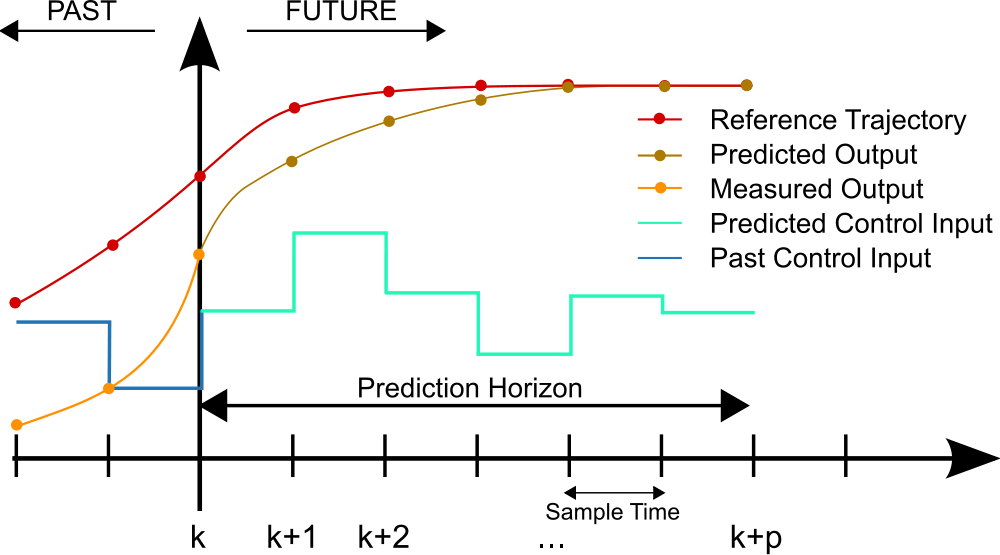
\includegraphics[width=0.85\textwidth,scale=1]{"src/Images/mpc.png"}
	\caption{A simple MPC Scheme \cite{MPC2023}}
	\label{fig:MPC Schematic}
\end{figure}

\clearpage

\subsection{Optimal Control Problems(OCP)}
An optimal control problem involves the mathematical formulation and analysis of determining an optimal trajectory for a dynamic system, subject to constraints and other performance criteria (minimizing the cost function). The OCP for a non-linear system with a quadratic cost function and constraints is as follows: 

\begin{equation}
\underset{\substack{x_0,x_1...x_N \\ u_0,u_1...u_{N-1}}} {\operatorname{min}} \sum_{k=0}^{N-1}\left (x_{k}^{T} Q x_{k}+ u_{k}^{T} R u_{k}\right)+x_{N}^{T} Q_f x_{N}^{T}
\end{equation}

\begin{equation}
\begin{array}{ll}
\text { subject to } & x_{k+1} = f(x_k,u_k)  \\
& x_0 = x(0) \\

& u_k \in \mathbb{U}, x_k \in \mathbb{X} \\

& \forall k \in[0, N-1] \\

& x_N \in \mathbb{X}_f \\
\end{array}
\end{equation}

Where $x_k$ and $u_k$ are the states and inputs respectively of the $k$-th time step and $x_N$ denotes the terminal state.

$Q$ and $R$ matrices are the state and input weight matrices respectively and $Q_f$ is the weight of the terminal state.

 

The constraints include the regular state and input constraints along with the dynamic model of the system as an additional continuity constraint. 

The cost function can be extended to include a different goal state by replacing the $x_k$ term with $(x_k - x_{goal})$.

\subsection{Stability}

While no concrete stability guarantees for Non-Linear MPC (NMPC) can be made, the theory behind Linear MPC has been well established for some time.This can be in practice adapted to NMPC.

The stability analysis of Linear MPC can be divided mainly into two parts :

\textbf{a. Recursive Feasibility}: Since the MPC algorithm involves the solution of an Optimization problem at every time step, one has to ensure that the problem remains feasible. This is done by proper choice of terminal sets. If the terminal set is chosen to be control invariant, one can ensure recursive feasibility. Written down mathematically, if  $\forall x \in \mathbb{X}_f \; \exists \;  \kappa(x) \in \mathbb{U} $ such that  $ f(x, \kappa(x)) \in \mathbb{X}_f $, then one can achieve recursive feasibility \cite{Fang2022, Allgower2004}. 

\textbf{a. Stability of the Origin}: Stability of the MPC algorithm in inherently tied to the choice of the terminal ingredients of the OCP. Recursive feasibility was achieved by selecting a suitable terminal set and likewise the stability at the origin can be confirmed by the right choice of terminal weights. 
A possible choice of terminal set is as follows: 

For positive definite $Q$ and $R$ matrices, solve the infinite horizon LQR problem. Since the infinite horizon LQR results in a constant quadratic optimal cost $P$, this can be assigned as the terminal weight to ensure stability about the origin \cite{Fang2022,Rawlings2017,Allgower2004}.

\subsection{Optimality}

Good choices of terminal ingredients can lead to stability. But sub-optimalities can arise due to the choice of prediction horizon and for any given initial condition there exists a prediction horizon $N_{min}$ that is optimal for the constrained closed loop system.

Any solution that satisfies the constraints is termed to be a feasible solution, whereas the feasible solution with the least cost is called the Optimal solution. 
For any prediction horizon, $N > N_{min}$ the performance of the closed loop does not visibly improve, and if  $N < N_{min}$ and the optimization problem is feasible, the closed loop can still be close to optimality because of the receding horizon (feedback) implementation.
 

  
\clearpage

